\documentclass[11pt,a4paper,ngerman]{article}
\usepackage[bottom=2.5cm,top=2.5cm]{geometry} 
\usepackage{babel}
\usepackage[utf8]{inputenc} 
\usepackage[T1]{fontenc} 
\usepackage{ae} 
\usepackage{amssymb} 
\usepackage{amsmath}
\usepackage{amsthm} 
\usepackage{graphicx}
\usepackage{fancyhdr}
\usepackage{fancyref}
\usepackage{listings}
\usepackage{xcolor}
\usepackage{paralist}

\usepackage[pdftex, bookmarks=false, pdfstartview={FitH}, linkbordercolor=white]{hyperref}
\usepackage{fancyhdr}
\pagestyle{fancy}
\fancyhead[C]{Computational Geometry}
\fancyhead[L]{Exercise sheet 4}
\fancyhead[R]{SoSe 2013}
\fancyfoot{}
\fancyfoot[L]{}
\fancyfoot[C]{\thepage \hspace{1px} of \pageref{LastPage}}
\renewcommand{\footrulewidth}{0.5pt}
\renewcommand{\headrulewidth}{0.5pt}
\setlength{\parindent}{0pt} 
\setlength{\headheight}{0pt}

\date{}
\title{Exercise sheet 4}
\author{Max Wisniewski, Alexander Steen}


%%
%% Enviroments for proofs and lemmas
%%
\newtheorem{lemma}{\bfseries Claim}

\begin{document}

\lstset{language=Pascal, basicstyle=\ttfamily\fontsize{10pt}{10pt}\selectfont\upshape, commentstyle=\rmfamily\slshape, keywordstyle=\rmfamily\bfseries, breaklines=true, frame=single, xleftmargin=3mm, xrightmargin=3mm, tabsize=2, mathescape=true}

\renewcommand{\figurename}{Figure}

\maketitle
\thispagestyle{fancy}

%%%%%%%%%%%%%%%%%%%%%%%%
%% Aufgabe 1 
%%%%%%%%%%%%%%%%%%%%%%%%
\subsection*{Task 1}

\subsubsection*{(a)}
Given a DCEL and one of its halfedges $\overrightarrow{e}$, which of the following are alway true?
\begin{itemize}
    \item 
        \begin{equation*}
            \text{Twin}(\text{Twin}(\overrightarrow{e})) = \overrightarrow{e}
        \end{equation*}
        is always true. Let $(a,b) = \overrightarrow{e}$ where $a,b \in V$.
        Then $\text{Twin}((a,b)) = (b,a)$ and therfor 
        \begin{equation*}
            \text{Twin}(\text{Twin}((a,b))) = \text{Twin}((b,a)) = (a,b)
        \end{equation*}
    \item
        \begin{equation*}
            \text{Next}(\text{Prev}(\overrightarrow{e})) = \overrightarrow{e}
        \end{equation*}
        is always True. We know that \emph{IncidentFace} for all $\overrightarrow{e}$, Next$(\overrightarrow{e})$,
        Prev$(\overrightarrow{e})$ is the same. \emph{Prev} is the previous edge walking around with the face on the left.
        \emph{Next} is the next one. Because there is only one traverse arround the face. Due to this unprecise definition
        this is a unprecise proof.
    \item
        \begin{equation*}
            \text{Twin}(\text{Prev}(\text{Twin}(\overrightarrow{e}))) = \text{Next}(\overrightarrow{e})
        \end{equation*}
        is not always true.
        Consider the example in Figure \ref{alge:ueb4:counter1.3}.
        \begin{figure}[bth]
            \centering
            \includegraphics[width=0.5\textwidth, clip, trim = 5cm 20cm 4cm 2cm]{media/counter13}
            \caption{Counter example for third assumption.}
            \label{alge:ueb4:counter1.3}
        \end{figure}

        We see that both edges are not the same.
    \item
        \begin{equation*}
            \text{IncidentFace}(\overrightarrow{e}) = \text{IncidentFace}(\overrightarrow{e})
        \end{equation*}
        is always true.

        This is true, because in \emph{de Berg et al.} \emph{Next} is defined this way.
\end{itemize}

\subsubsection*{(b)}

\begin{description}
    \item[All incident vertices:]\mbox{}
\begin{lstlisting}
allVertices(v Vertex)
    res := empty
    start := Prev(IncidentEdge(v))
    akt := start
    do{
        res.add(Origin(akt))
        akt := Prev(Twin(akt))
    } until (akt = start)
\end{lstlisting}
    This algorithm uses the shown error in Figure \ref{alge:ueb4:counter1.3} to swing itself around the vertex once.
    \item[All incident edges:]\mbox{}
\begin{lstlisting}
allEdges(f Face)
    toWork := OuterComponent(f) = nil ? empty : {OuterComponent(f)}
    res := empty
    forall( e : InnerComponents(f) ){
        toWork.add(Twin(e))
    }
    forall(e : toWork){
        e' := e
        do{
            res.add(e')
            e' := Next(e)
        } until (e = e')
    }
    return res
\end{lstlisting}
We didn't know, if the edges from \emph{InnerComponents} have the face to the
hole or to the face $f$. If it is the other way around remove \emph{Twin} from line
4. Otherwise a face gives us for the sourrounding and each hole one edge, over which we iterate
and collect all edges.
\end{description}

\subsection*{Task 2}

tbd

\subsection*{Task 3}

Let $P$ be a set of $n$ points in the plane such that no two points in $P$ have the same x-coordinate
and such that no three points in $P$ are collinear. A \emph{triangulation} $T$ of $P$ is a maximal planar
straight-line graph with vertex set $P$.

\subsubsection*{(a)}

Let $T$ be a triangulation of $P$. Show that all the bounded faces of $T$ are triangles and that 
the unbounded face is the exterior of the convex hull of $P$.\\

\textbf{Proof.}\\

First, there is only one unbounded face. If this was not the case two of the unbounded
faces have to be seperated by a line. This line as at most one endpoint and is infinite
on the other one. Therefor this cannot be a line with endpoints in $P$.\\

There is no edge into the convex hull, because there are no points of $P$ in there. Therefor
the unbounded face contains at least the exterior of the convex hull.

Assume the unbounded face contains more then the convex hull. Then there is a area sourrounded by
at least three points of $P$ connected to the conves hull. But then there exists a straight line
between at least two of these points because otherwise the area would not be open. Hence $T$ was
not maximal.\\

Last we show that the inside consists only of triangles. Suppose this was not the case,
then there would be some simple polygon $G$ with $n \geq 4$ points. It is simple because
the lines are not crossing in $T$. We know there is a triangulation for $G$ that adds at least one
diagonal. Hence $T$ was not maximal.
\mbox{}\hfill $\square$

\subsubsection*{(b)}

Give an algorithm that finds a triangulation of $P$ in $O(n \log n)$ time.\\

\textbf{Solution.}\\

\begin{lstlisting}
triangle(P)
    sort(P,x)
    left <- min(P)
    P1, P2 <-split(P,left.y)
    left := false
    for (p : { P1, P2 })
        left := not left
        edges <- (p[0], p[1])
        stack.add(p[0],p[1])
        for(i := 2 to |p|)
            edges.add(p[i-1],p[i])
            qlast := stack.pop
            while(right(stack.top,qlast,p[i]) && left || not(left) && left(stack.top,qlast,p[i]))
                diagonals.add(stack.top,p[i])
                qlast := stack.pop
    edges.add(P1[|P1|],P2[|P2|])
    triangulate(P1,P2, edges)
    return diagonals
\end{lstlisting}

We sort every point by their x-coordinate. We take the left most one and partition $P$ by that ones y-coordinate.
Then we connect the points in $P1$ and $P2$. If in P1 (lower part) we do a right turn, we connect the last point on the convex hull
with this point. In P2 the other way arround.

We get a y-monoton polygon with $P$ and \lstinline|edges| and the exterior of this one bounded by the convex hull is triangulated at this point.
Then we triangulate the y-monoton polygon.\\

\textbf{Running time:}\\
The sorting costs $O(n \log n)$ the connecting of the edges takes $O(n)$ as we have shown for already sorted convex hull computation.
The points in P1 and P2 are already sorted and the polygon is y-monoton, therefor the triangulation of this part takes $O(n)$ time.\\

The total running time is in $O(n \log n)$.\\

\textbf{Correctness:}\\
The algroithm is correct. The only part missing is, that the area between convex hull and y-monoton part is triangulated.

Assume there is a face $f$, that is not a triangle. We iterated over the points in x-coordinate and there are no three points on a line.
We know this polygon $f$ can be triangulated. Take one diagonal from the triangulation. Assume w.l.o.g that we are on P1. Then
there is a point on the left of this diagonal (otherwise this diagonal would be an edge of the y-monoton polygon).

Hence the point is on the left of the diagonal the algorithm would have put at least one diagonal (if there is no other this one) into the
triangulation. We conclude that this could not be a triangulation calculated by our algorithm.

\label{LastPage}


\end{document}
